 %!TeX root = Project 1 Math 5.tex
\documentclass{article}
\usepackage[dvipsnames, svgnames, x11names]{xcolor}
\usepackage{tikz}
\usetikzlibrary{automata, positioning, arrows}
\usepackage{pgfplots}
\usepackage{setspace}
\usepackage{units}
\usepackage{graphicx}
\usepackage{amsopn}
\usepackage{bbding}
\usepackage{amsmath}
\usepackage{hyperref}
\usepackage{cancel}
\usepackage{gensymb}
\usepackage[margin = 1in]{geometry}
\title{Project 2, Matrix Algebra, Markov Chains}
\date{25 March, 2025}
\author{Tejas Patel}
\begin{document}
\maketitle
\section{}
Matrices Defined: $x_0=\begin{bmatrix}0.2\\0.2\\0.6\end{bmatrix}$, $A=\begin{bmatrix}0.98&0.05&0.05\\0.01&0.9&0.16\\0.01&0.05&0.79\end{bmatrix}$
\subsection*{a: State Diagram}
$\begin{bmatrix}&R&C&D\\R&0.98&0.05&0.05\\C&0.01&0.9&0.16\\D&0.01&0.05&0.79\end{bmatrix}$
\\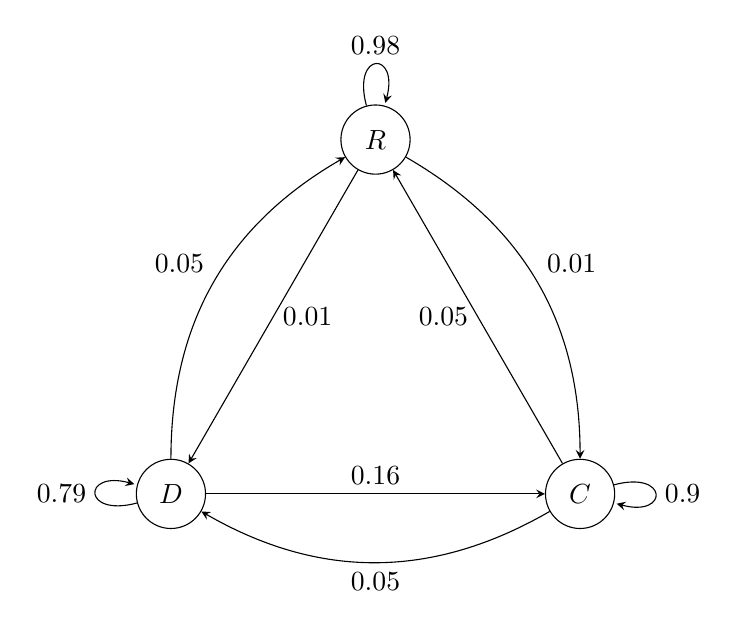
\begin{tikzpicture}[->, >=stealth, auto]
    \foreach \angle/\name in {90/R, -30/C, 210/D} {
      \node[state] (\name) at (\angle:3cm) {$\name$};
    }
    \draw (R) edge[bend left] node{0.01} (C)
          (R) edge[right] node{0.01} (D)
          (R) edge[loop above] node{0.98} (R)
          (C) edge[bend left] node{0.05} (D)
          (C) edge[left] node{0.05} (R)
          (C) edge[loop right] node{0.9} (C)
          (D) edge[above] node{0.16} (C)
          (D) edge[bend left] node{0.05} (R)
          (D) edge[loop left] node{0.79} (D);
\end{tikzpicture}
\subsection*{b: }
The weight of $D \rightarrow C$ is 0.16, meaning 16\% of disposable cup users will switch to compostable cups
\subsection*{c: }
$\vec{x_1}=\begin{bmatrix}0.98&0.05&0.05\\0.01&0.9&0.16\\0.01&0.05&0.79\end{bmatrix}\begin{bmatrix}0.2\\0.2\\0.6\end{bmatrix} = \begin{bmatrix}0.2*0.98+0.2*0.05+0.6*0.05\\0.2*0.01+0.2*0.9+0.6*0.16\\0.2*0.01+0.2*0.05+0.6*0.79\end{bmatrix}=\begin{bmatrix}0.236\\0.278\\0.486 \end{bmatrix}$
\\This means after the first year passes, 23.6\% of people use Recyclable cups, 27.8\% use compostable, and 48.6\% of people use disposable cups
\pagebreak
\subsection*{d: Computed using SageMath:}
\textbf{}
\begin{tabular}{c|c|c|c|c|c|c|c|c}
    $\vec{x_1}$&$\vec{x_2}$&$\vec{x_3}$&$\vec{x_4}$&$\vec{x_5}$&$\vec{x_6}$&$\vec{x_7}$&$\vec{x_8}$&$\vec{x_9}$ \\ \hline
    \\$\begin{bmatrix}0.236\\0.278\\0.486 \end{bmatrix}$ & $\begin{bmatrix}0.2695 \\ 0.3303 \\0.4002\end{bmatrix}$ & $\begin{bmatrix}0.3006 \\ 0.3640 \\0.3354\end{bmatrix}$ & $\begin{bmatrix}0.3296 \\ 0.3843 \\0.2861\end{bmatrix}$ & $\begin{bmatrix}0.3565 \\ 0.3949 \\0.2486\end{bmatrix}$ & $\begin{bmatrix}0.3815 \\ 0.3988 \\0.2197\end{bmatrix}$ & $\begin{bmatrix}0.4048 \\ 0.3979 \\0.1973\end{bmatrix}$ & $\begin{bmatrix}0.4265 \\ 0.3937 \\0.1798\end{bmatrix}$ & $\begin{bmatrix}0.4466 \\ 0.3873 \\0.1660\end{bmatrix}$
\end{tabular}
\begin{center}
    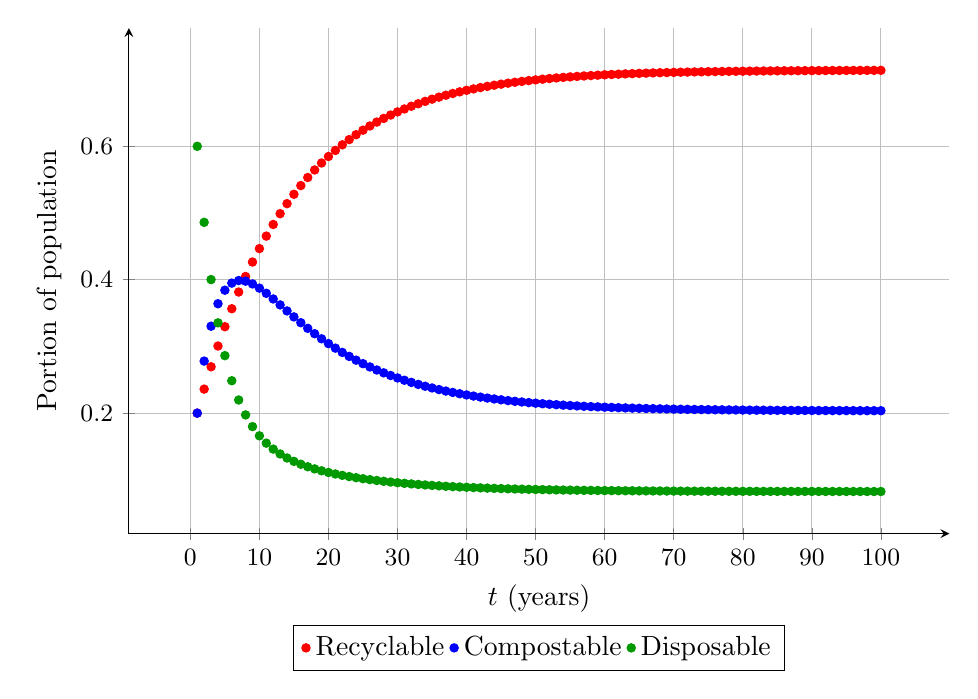
\begin{tikzpicture}
        \begin{axis}[
          xlabel={$t$ (years)},
          ylabel={Portion of population},
          axis lines=left,
          enlargelimits=true,
          width=12cm,
          height=8cm,
          grid=both,
          tick label style={font=\small},
          legend style={at={(0.5,-0.18)}, anchor=north, legend columns=3}
        ]
      
          % Dataset 1 - Red
          \addplot[
            only marks,
            mark=*,
            mark size=1.5pt,
            color=red
          ] coordinates {
            % Paste (x, y) points here
            (1,0.2)	(2,	0.236)(3,	0.26948)(4,	0.3006164)(5,	0.329573252)(6,	0.3565031244)(7,	0.3815479057)(8,	0.4048395523)(9,	0.4265007836)(10,	0.4466457287)(11,	0.4653805277)(12,	0.4828038908)(13,	0.4990076184)(14,	0.5140770851)(15,	0.5280916892)(16,	0.5411252709)(17,	0.553246502)(18,	0.5645192468)(19,	0.5750028996)(20,	0.5847526966)(21,	0.5938200078)(22,	0.6022526073)(23,	0.6100949248)(24,	0.61738828)(25,	0.6241711004)(26,	0.6304791234)(27,	0.6363455848)(28,	0.6418013938)(29,	0.6468752963)(30,	0.6515940255)(31,	0.6559824437)(32,	0.6600636727)(33,	0.6638592156)(34,	0.6673890705)(35,	0.6706718356)(36,	0.6737248071)(37,	0.6765640706)(38,	0.6792045856)(39,	0.6816602646)(40,	0.6839440461)(41,	0.6860679629)(42,	0.6880432055)(43,	0.6898801811)(44,	0.6915885684)(45,	0.6931773686)(46,	0.6946549528)(47,	0.6960291061)(48,	0.6973070687)(49,	0.6984955739)(50,	0.6996008837)(51,	0.7006288219)(52,	0.7015848043)(53,	0.702473868)(54,	0.7033006973)(55,	0.7040696485)(56,	0.7047847731)(57,	0.705449839)(58,	0.7060683502)(59,	0.7066435657)(60,	0.7071785161)(61,	0.70767602)(62,	0.7081386986)(63,	0.7085689897)(64,	0.7089691604)(65,	0.7093413192)(66,	0.7096874268)(67,	0.710009307)(68,	0.7103086555)(69,	0.7105870496)(70,	0.7108459561)(71,	0.7110867392)(72,	0.7113106674)(73,	0.7115189207)(74,	0.7117125963)(75,	0.7118927145)(76,	0.7120602245)(77,	0.7122160088)(78,	0.7123608882)(79,	0.712495626)(80,	0.7126209322)(81,	0.7127374669)(82,	0.7128458443)(83,	0.7129466352)(84,	0.7130403707)(85,	0.7131275447)(86,	0.7132086166)(87,	0.7132840134)(88,	0.7133541325)(89,	0.7134193432)(90,	0.7134799892)(91,	0.71353639)(92,	0.7135888427)(93,	0.7136376237)(94,	0.71368299)(95,	0.7137251807)(96,	0.7137644181)(97,	0.7138009088)(98,	0.7138348452)(99,	0.713866406)(100,	0.7138957576)
          };
          \addlegendentry{Recyclable}
      
          % Dataset 2 - Blue
          \addplot[
            only marks,
            mark=*,
            mark size=1.5pt,
            color=blue
          ] coordinates {
            % Paste (x, y) points here
            (1,0.2)	(2,	0.278)(3,	0.33032)(4,	0.3640148)(5,	0.384278492)(6,	0.3949300963)(7,	0.3987728026)(8,	0.3978596881)(9,	0.3936902363)(10,	0.3873556573)(11,	0.3796463271)(12,	0.3711312029)(13,	0.3622165065)(14,	0.3531890721)(15,	0.3442483506)(16,	0.335530026)(17,	0.3271234286)(18,	0.3190843619)(19,	0.3114445408)(20,	0.3042185252)(21,	0.2974088042)(22,	0.2910095139)(23,	0.2850091492)(24,	0.2793925317)(25,	0.2741422315)(26,	0.2692395862)(27,	0.2646654253)(28,	0.260400577)(29,	0.2564262179)(30,	0.2527241068)(31,	0.2492767352)(32,	0.2460674175)(33,	0.243080338)(34,	0.2403005678)(35,	0.2377140596)(36,	0.2353076288)(37,	0.2330689242)(38,	0.2309863933)(39,	0.2290492432)(40,	0.2272474003)(41,	0.2255714693)(42,	0.2240126928)(43,	0.2225629119)(44,	0.2212145276)(45,	0.2199604652)(46,	0.2187941389)(47,	0.2177094199)(48,	0.2167006048)(49,	0.2157623872)(50,	0.2148898305)(51,	0.214078342)(52,	0.2133236498)(53,	0.2126217802)(54,	0.2119690371)(55,	0.2113619829)(56,	0.2107974201)(57,	0.2102723749)(58,	0.2097840816)(59,	0.2093299678)(60,	0.2089076413)(61,	0.2085148772)(62,	0.2081496061)(63,	0.2078099037)(64,	0.2074939803)(65,	0.2072001714)(66,	0.2069269289)(67,	0.2066728134)(68,	0.2064364859)(69,	0.2062167012)(70,	0.2060123015)(71,	0.2058222097)(72,	0.2056454243)(73,	0.2054810138)(74,	0.2053281121)(75,	0.2051859135)(76,	0.2050536688)(77,	0.2049306813)(78,	0.2048163028)(79,	0.2047099309)(80,	0.2046110049)(81,	0.2045190038)(82,	0.2044334428)(83,	0.204353871)(84,	0.2042798693)(85,	0.2042110477)(86,	0.2041470436)(87,	0.2040875197)(88,	0.2040321626)(89,	0.2039806804)(90,	0.203932802)(91,	0.2038882751)(92,	0.2038468651)(93,	0.2038083538)(94,	0.2037725382)(95,	0.2037392298)(96,	0.2037082529)(97,	0.2036794445)(98,	0.2036526526)(99,	0.2036277361)(100,	0.2036045638)	
          };
          \addlegendentry{Compostable}
      
          % Dataset 3 - Green
          \addplot[
            only marks,
            mark=*,
            mark size=1.5pt,
            color=green!60!black
          ] coordinates {
            % Paste (x, y) points here
            (1,0.6)	(2,	0.486)(3,	0.4002)(4,	0.3353688)(5,	0.286148256)(6,	0.2485667794)(7,	0.2196792918)(8,	0.1973007597)(9,	0.1798089801)(10,	0.1659986139)(11,	0.1549731451)(12,	0.1460649063)(13,	0.138775875)(14,	0.1327338428)(15,	0.1276599603)(16,	0.123344703)(17,	0.1196300694)(18,	0.1163963913)(19,	0.1135525597)(20,	0.1110287782)(21,	0.108771188)(22,	0.1067378788)(23,	0.104895926)(24,	0.1032191883)(25,	0.1016866681)(26,	0.1002812904)(27,	0.09898898995)(28,	0.09779802917)(29,	0.09669848583)(30,	0.09568186767)(31,	0.09474082105)(32,	0.09386890983)(33,	0.09306044637)(34,	0.09231036169)(35,	0.09161410483)(36,	0.09096756415)(37,	0.09036700519)(38,	0.08980902102)(39,	0.08929049213)(40,	0.08880855359)(41,	0.08836056781)(42,	0.08794410166)(43,	0.08755690701)(44,	0.08719690394)(45,	0.08686216618)(46,	0.08655090823)(47,	0.08626147398)(48,	0.0859923265)(49,	0.08574203886)(50,	0.0855092858)(51,	0.08529283614)(52,	0.08509154587)(53,	0.08490435177)(54,	0.08473026559)(55,	0.08456836865)(56,	0.08441780686)(57,	0.08427778615)(58,	0.0841475682)(59,	0.08402646646)(60,	0.08391384255)(61,	0.08380910284)(62,	0.0837116953)(63,	0.08362110658)(64,	0.08353685928)(65,	0.08345850945)(66,	0.08338564423)(67,	0.08331787966)(68,	0.08325485867)(69,	0.08319624919)(70,	0.08314174242)(71,	0.08309105115)(72,	0.08304390828)(73,	0.08300006543)(74,	0.08295929159)(75,	0.08292137193)(76,	0.08288610664)(77,	0.08285330994)(78,	0.082822809)(79,	0.08279444313)(80,	0.08276806288)(81,	0.08274352924)(82,	0.08272071296)(83,	0.08269949382)(84,	0.08267976002)(85,	0.08266140759)(86,	0.08264433983)(87,	0.08262846681)(88,	0.0826137049)(89,	0.08259997632)(90,	0.08258720875)(91,	0.08257533491)(92,	0.08256429223)(93,	0.08255402255)(94,	0.08254447174)(95,	0.08253558948)(96,	0.08252732899)(97,	0.08251964673)(98,	0.08251250223)(99,	0.08250585784)(100,	0.08249967856)
        
          };
          \addlegendentry{Disposable}
      
        \end{axis}
      \end{tikzpicture}
\end{center}
\subsubsection*{Observations}
The percentage of people using Recyclable cups increases at a decreasing rate, compostable cups go up then start dropping, and disposable decreases at a decreasing rate
\subsection*{e:}
After infinite time, the portion of the population using each type of cup came to the following:
\\\textbf{Recyclable:} $\frac{130}{182}$ of the population, or about 71.43\%
\\\textbf{Compostable:} $\frac{37}{182}$ of the population, or about 20.33\%
\\\textbf{Disposable:} $\frac{15}{182}$ of the population, or about 8.24\%
\end{document}

